%% 
%% 
%% 

\section{Experiments}
\label{sec:exp}
\vspace{-2mm}

\begin{figure*}[h]
  \centering
  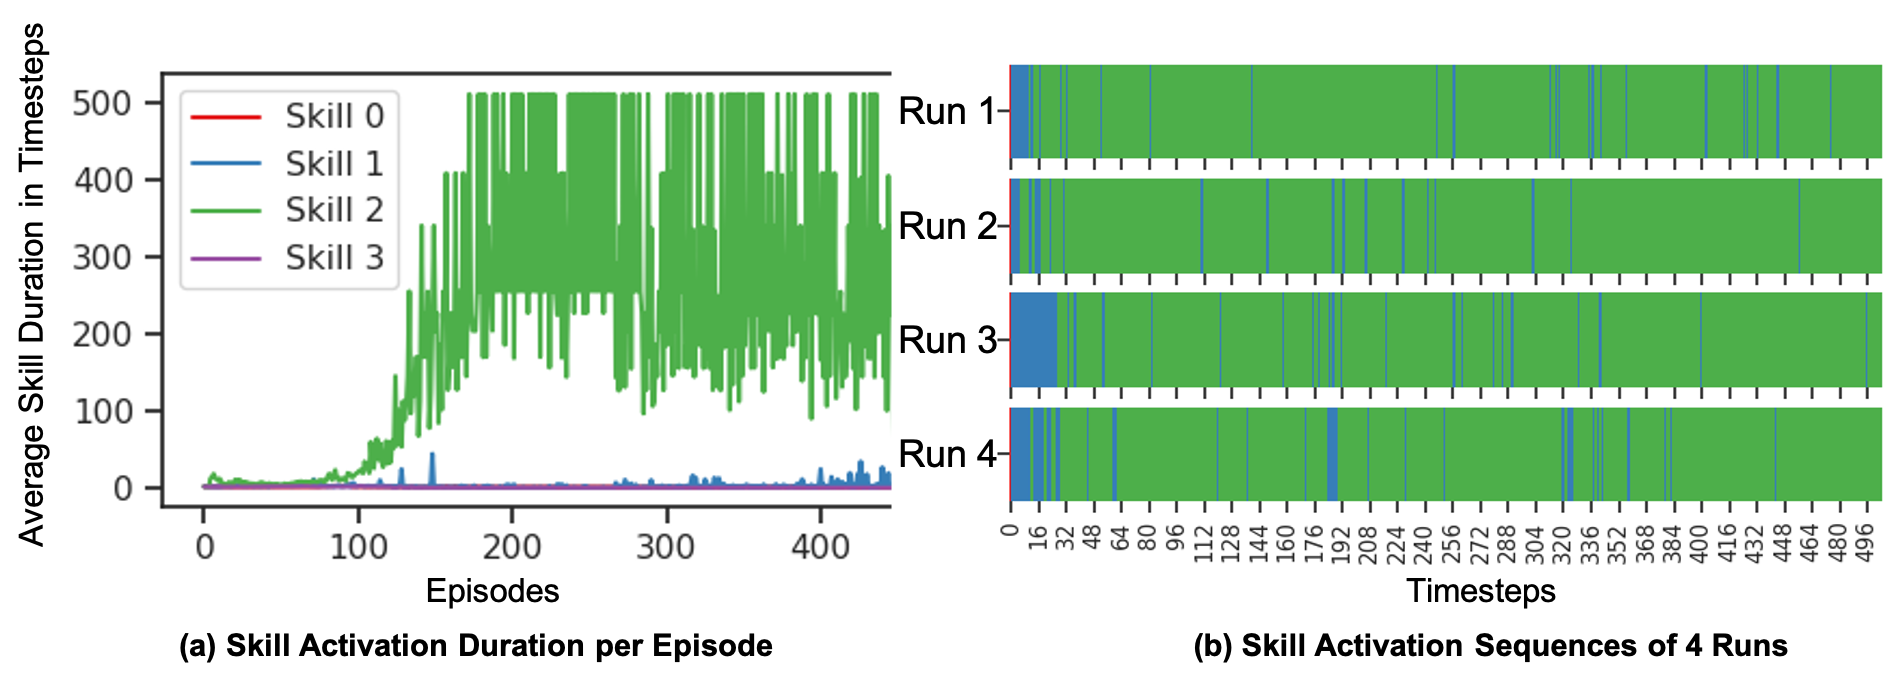
\includegraphics[width=0.7\linewidth]{./Part1/figures/skill_sequence_joint.png}\\
  \vspace{-4mm}\caption{\label{fig:skill_sequence} Skill Duration
  Patterns}\vspace{-3mm}
\end{figure*}
\begin{figure*}[h]
  \centering
  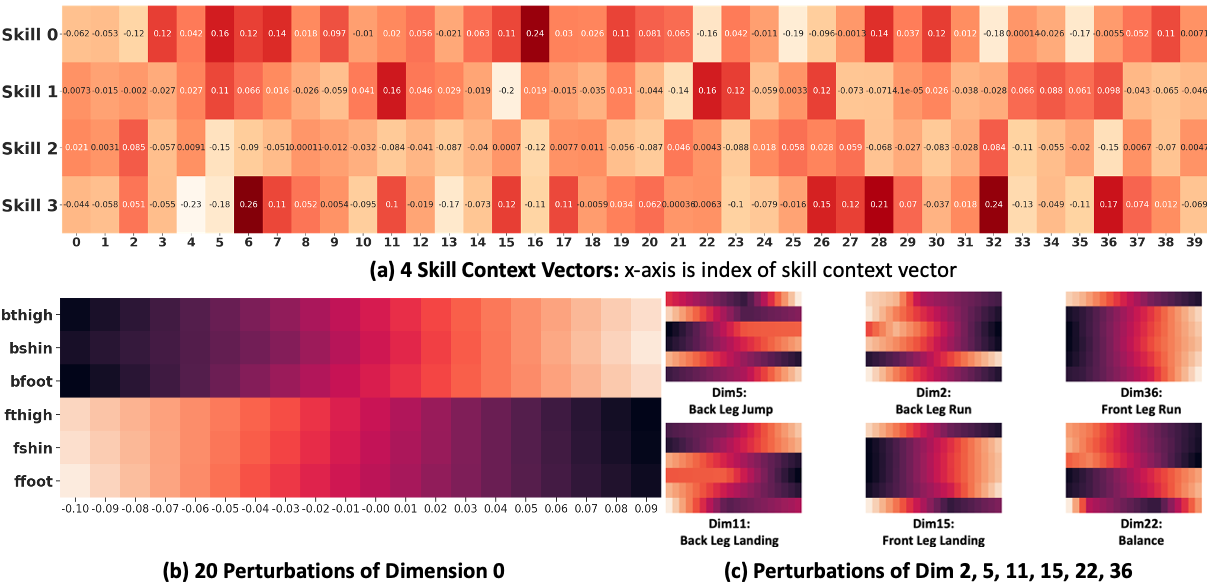
\includegraphics[width=0.75\linewidth]{./Part1/figures/Interp_joint.png}\\
  \vspace{-4mm}\caption{\label{fig:interp_joint} Interpretation
    of Skill Context Vectors}\vspace{-4mm}
\end{figure*}

% to write: in this section,
In this section, we design experiments to answer three questions:
1) Can SA outperform other baselines (regarding episodic returns,
stability, and scalability)? 2) Can SA temporally extend skills
without the termination function? 3) Can skill context vectors be
easily interpreted? 4) Does skill embeddings learned by SA have a
performance boost over other option variants in transfer learning
settings?

For single task learning, experiments are conducted on all OpenAI
Gym MuJoCo environments (10 environments)
\cite{brockman2016openai}. We follow DAC~\cite{zhang2019dac} and
compare our algorithm with five baselines, four of which are
option implementations, i.e., DAC+PPO \cite{zhang2019dac},
AHP+PPO \cite{levy2011unified}, PPOC
\cite{klissarov2017learnings} and OC \cite{bacon2017option}. The
last baseline is PPO \cite{schulman2017proximal}. All baselines'
parameters used in DAC\footnote{All baselines' implementations
  are from DAC's open source repo
  https://github.com/ShangtongZhang/DeepRL/tree/DAC. Note that
  the author list of this paper does not have any overlap with
  DAC. Our source code is available in supplementary materials.}
remain unchanged other than the maximum number of training steps:
SA only needs 1 million steps to converge rather than the 2
million used in DAC. For transfer learning, we follow
\citename{zhang2019dac} and run 6 pairs of transfer learning
tasks constructed in DAC based on DeepMind Control Suite
\cite{tassa2020dmcontrol}. For a fair comparison, we use four
skills for SA and four options for other option implementations.
All experiments are run on an Intel® Core™ i9-9900X CPU @ 3.50GHz
with a single thread and process. Our implementation details are
summarized in Appendix~\ref{sec:append_implement}.

\begin{figure*}[h]
  \vspace{-2mm}
  \centering
  \includegraphics[width=1\linewidth]{./Part1/figures/transfer.png}\\
  \vspace{-4mm}
  \caption{\label{fig:transfer} Performance on DAC transfer
    learning tasks}
  \vspace{-4mm}
\end{figure*}

\subsection{Single Task Learning}
\label{sec:exp_perf}
\vspace{-2mm}
% towrite: figure capitalize
In Figure~\ref{fig:exp_dac}, we report episodic returns on
infinite horizon and finite horizon\footnote{We refer to
  environments with the game-over condition as finite horizon
  environments, and infinite vice versa.} environments
separately. For a fair comparison, we use exactly the same
plotting script as used in DAC: curves are averaged over 10
independent runs and smoothed by a sliding window of size 20.
Shaded regions indicate standard deviations. Performance of all
ten environments is shown in (Appendix
Figure~\ref{fig:all_tasks}, Table~\ref{table:single_infinite}).

It is extremely interesting that SA shows two completely
different kinds of behaviors on infinite and finite horizon
environments. According to previous option framework
implementations~\cite{klissarov2017learnings,smith2018inference,harb2018waiting,zhang2019dac},
on single task environments, option-based algorithms do not have
a distinguishable performance boost over hierarchy-free
algorithms. SA also has similar behavior and achieves comparable
performance to the best baseline algorithm on most finite horizon
environments (Figure~\ref{fig:exp_dac} (b)). In
Appendix~\ref{sec:append_gist} we conceptually explain that
conventional value functions are insufficient to approximate
models which have temporal latent variables dependencies. A
concrete deep wide skill-action architecture remains open for the
future work.

On infinite horizon environments as shown in
Figure~\ref{fig:exp_dac} (a), SA's performance significantly
outperforms all baselines by a large margin in various aspects.
For episodic return, e.g., HumanoidStandup, all option
implementations barely converge, while SA is $240\%$ better than
DAC and AHP\footnote{Even on Reacher, a simple environment on
  which most algorithms converge to a similar performance, SA is
  still $38\%$ better than the second best (AHP).}. For
convergence, SA has the fastest convergence speed. On the first
two environments, which are also reported in DAC, SA only takes
$40\%$ of time steps of DAC and AHP to reach similar episodic
returns. This acceleration is because: 1) SA is MDP formulated,
the skill policy is updated at each time step; 2) SA only has one
action policy decoder; 3) the action decoder learns to decode
skill context vectors whichever skill is activated. For
stability, all 10 runs of SA converge to a similar level while
the other have much larger standard deviations. This property is
theoretically justified by Proposition~\ref{prop:var_red} and
further discussed in Appendix~\ref{sec:append_gist}.

\vspace{-2mm}
\subsection{Temporal Extension}
\label{sec:exp_ext}

It is logical to ask whether SA is capable of temporal extension
without the termination function. To illustrate this, we plot the
average duration of each skill during training episodes of the
HalfCheetah environment in Figure~\ref{fig:skill_sequence} (a)
and 4 runs of skill activation sequences in
Figure~\ref{fig:skill_sequence} (b). (more details in
Appendix~\ref{sec:append_exp_ext}). At the start of training, all
skills' durations are short, while Skill 2's duration quickly
grows and dominates the entire episode. This growth of duration
proves that SA can still temporally extend a skill. Towards the
end of the training, the dominant skill's duration starts to
decrease while the duration of a secondary skill (Skill 1) starts
to increase. This means that during later training stages, SA
starts to coordinate different skills. The dominant skill
phenomenon is also reported in other option implementations such
as DAC. However, as shown in the
video\footnote{https://www.youtube.com/watch?v=QiLVZvI6NJU}, SA
still learns distinguishable skills. Skill 2 is the running
forward skill thus it dominates the whole episode. Skill 1 is
only used to recover from falling down thus it has much shorter
duration. As discussed in Appendix \ref{sec:append_gist},
solution to the dominant skill is actually learning skills at
much finer granularity. The SA-style wide value function
(Eq.~(\ref{eq:sa_v})) provides an elegant solution to this
problem.

\vspace{-2mm}
\subsection{Interpretation of Skill Context Vectors}
\label{sec:interpret}

Explicit skill representations not only improve efficiency,
scalability, and generalization, but also benefit interpretation.
We continue with the HalfCheetah example and demonstrate how
easily skill context matrix $\mW_s$
(Figure~\ref{fig:interp_joint} (a)) can be interpreted (more
details are provided in Appendix~\ref{sec:append_interpret}). We
first follow \citename{sabour2017dynamic} and interpret what
property is represented by a context vector's dimension by adding
perturbations on to it, and inspecting perturbations' effects
on the action policy decoder in generating primary actions $\rva$
(Figure~\ref{fig:interp_joint} (b)). Once each dimension is
understood, skills become straight forward to interpret by simply
inspecting on which dimensions (property) each skill $\hat{\rvo}$
in Figure ~\ref{fig:interp_joint} (a) has significant weights,
and interpreting properties of those dimensions
((Figure~\ref{fig:interp_joint} (c)). In this way, we can
interpret that Skill 2 is a forward movement skill, since it
focuses on jumping and running forward, while Skill 1 is a
landing skill. These interpretations can further be used to
explain skill activation patterns in
Figure~\ref{fig:skill_sequence} (b): Skill 2 has the longest
duration because it is the major source of all forward movements.
Skill 2 occasionally falls back to Skill 1 because, after jumping
or running, the HalfCheetah needs to land and balance itself.


\subsection{Transfer Learning}
\label{sec:transfer}

We follow \citename{zhang2019dac} and run 6 pairs of transfer
learning tasks constructed in DAC based on DeepMind Control Suite
\cite{tassa2020dmcontrol}. Each pair contains two different
tasks. To keep consistent with DAC, we train all models one
million steps on the first task and switch to the second (SA's
skill context matrix is subsequently frozen) to run another one
million steps. Results are reported in Figure~\ref{fig:transfer}
(Appendix Table~\ref{table:transfer}). On the first task, SA's
performance is among the best algorithms in all environments.
This further validates SA's advantages on single task as observed
in section~\ref{sec:exp_perf}. On the transfer learning (the
second) task, SA's performance ranks the first in 5 out of 6
environments. This shows SA's advantages in knowledge reuse
tasks. \vspace{-2mm}

\section{Conclusions}
\label{sec:conclusion}
\vspace{-2mm}

In this paper, we presented a novel MDP equivalence of the SMDP
formulated option framework, from which an MDP implementation of
the option framework, i.e., the Skill-Action architecture, was
derived. We theoretically proved that SA has lower variance than
conventional RL models and provided policy gradient theorems for
updating SA. Our empirical studies on challenging infinite
horizon robot simulation environments demonstrated that SA not
only outperforms all baselines by a large margin, but also
exhibits smaller variance, faster convergence, and good
interpretability. On transfer learning, SA also outperforms the
other models in 5 out of 6 environments and shows its advantages
in knowledge reuse tasks.

The final and most important contribution of SA is hierarchically
learning explicit abstract actions' representations with ``skill
context vectors''. This design significantly improves the
scalability and interpretability of SA. It is straightforward to
extend SA to deeper and wider (Appendix~\ref{sec:append_gist})
architectures, which gives rise to a large-scale pre-training and
transfer learning architecture in the reinforcement learning
area.

Experiments also show that SA shares two innate limitations with
the conventional option framework
\cite{levy2011unified,klissarov2017learnings,smith2018inference,harb2018waiting,zhang2019dac}:
(1) failure to improve the performance and the sample efficiency
on finite horizon environments (section~\ref{sec:exp_perf}); (2)
``the dominant skill problem'' \cite{zhang2019dac} (section
\ref{sec:exp_ext}). In Appendix~\ref{sec:append_gist} we
conceptually discuss that SA-style wide (higher-order
dependencies) value functions could be a solution to both
limitations. This is mainly because these limitations are caused
by the insufficiency of the conventional value functions in
approximating values that have temporal latent variables
dependencies (discussed in Appendix~\ref{sec:append_gist}).



%%% Local Variables:
%%% mode: latex
%%% TeX-master: "../thesis"
%%% End:
